\documentclass[aspectratio=169,cramped]{beamer}
\usetheme[minimal,infbio]{tugraz2018}
\usepackage[utf8]{inputenc}
\usepackage{booktabs}
\usepackage{varwidth,lipsum}
\newcommand\hide[1]{\phantom{\varwidth{\linewidth}#1\endvarwidth}}
\usepackage{ulem}
\usepackage[ttscaled=0.8,tt=false]{libertine}

\usepackage{tikz}
\usepackage{tikz-qtree}

\hypersetup{colorlinks,urlcolor=blue,linkcolor=}
\let\tempone\itemize
\let\temptwo\enditemize
\renewenvironment{itemize}{\tempone\addtolength{\itemsep}{-0\baselineskip}\addtolength{\parskip}{-0.2\baselineskip}}{\temptwo}
\newcommand{\putat}[3]{\begin{picture}(0,0)(0,0)\put(#1,#2){#3}\end{picture}}
\newcommand{\ex}[1]{{\color{teal} #1}}
\newcommand{\checkyes}{\textcolor{tuggreen}{\faCheckSquareO}}
\newcommand{\checkno}{\textcolor{black}{\faSquareO\,}}
\newcommand{\bulletplus}{\textcolor{tuggreen}{\faPlusCircle}}
\newcommand{\bulletminus}{\textcolor{tugred}{\faMinusCircle}}
\newcommand{\bulletconclusion}{\textcolor{tugblue}{\faArrowCircleRight}}

\title{Natural Language Processing: \\ How do humans process language?}
% \subtitle{Natural Language Processing}
\author{Philipp Gabler <pgabler@student.tugraz.at>}
\instituteurl{}
\date{2020-05-07}

\begin{document}

\begin{frame}
    \titlepage
\end{frame}

\begin{frame}{Outline}
    \tableofcontents
\end{frame}


%//////////////////////////////////////////////////////////////////////
\sectionheader[What does NLP have to do with humans, at all?]{\textbf{Motivation}}
\section{Motivation}

\begin{frame}{Fundamental questions of linguistics}
  \begin{itemize}
  \item What do you know when you know a language?
  \item What do you know when you understand an utterance?
  \end{itemize}
	
\end{frame}

\begin{frame}{Linguistics \& NLP}
  \textbf{Too much theory is bad? But why?}
	\begin{itemize}
  \item ``Every time I fire a linguist, the performance of the speech processing system goes up.''
    (Frederick Jelinek)
  \item Does it mean we should refrain from linguistic inspiration?
    \begin{itemize}
    \item (NLP already does that.  Ask a linguist.)
    \end{itemize}
  \item Cf. the good, bad, and ugly parts of artificial neural networks
	\end{itemize}
\end{frame}

\begin{frame}{Levels of Abstraction}
	\textbf{Linguists and Engineers tend to have different focus}
	\begin{itemize}
  \item Computational: what is explained?
    \begin{itemize}
    \item \ex{Description of linguistic performance vs. explanation of linguistic competence}
    \end{itemize}
  \item Algorithmic: how is it done?
    \begin{itemize}
    \item  \ex{Cognitive realism, computational complexity/efficiency}
    \end{itemize}
  \item Implementational: how is is realized?
    \begin{itemize}
    \item  \ex{Neurological plausibility}
    \end{itemize}
  \end{itemize}
\end{frame}

\begin{frame}{What this lecture is about}
	\textbf{A very short introduction to:}
	\begin{itemize}
  \item Grammar theory
    \begin{itemize}
    \item What is language built of?
    \end{itemize}
  \item Cognitive linguistics
    \begin{itemize}
    \item How does language work in the mind?
    \end{itemize}
  \end{itemize}
\end{frame}

\begin{frame}{Insights \textit{from} linguistics}
	\textbf{Get a better understanding of what should work in language processing}
	\begin{itemize}
  \item After all, it's \emph{natural language} processing
  \item Comparison gives confidence:
    \begin{itemize}
    \item NLU system behaviour vs. L1 acquisition
    \item Observation of similar effects/errors, e.g., garden path sentences
    \item Human performance is the ultimate (utopic?) benchmark!
    \item We're not inventing something \emph{new}\ldots
    \end{itemize}
  \end{itemize}
\end{frame}

\begin{frame}{Insights \textit{for} linguistics}
	\textbf{We don't yet know how human language really works}
	\begin{itemize}
  \item Very conflicting hypotheses, most of which work only on a computational level
  \item New ideas:
    \begin{itemize}
    \item Shallow processing
    \item Distributed, implicit, usage-based knowledge
    \item Computational construction grammar
    \item Computational semantics (\(\lambda\) calculus)
    \end{itemize}
  \end{itemize}
\end{frame}

\begin{frame}{Some words of caution}
  \textbf{Be warned!}
  \begin{itemize}
  \item This is will be an extremely rough, simplified, and incomplete overview
  \item It is biased in favour of Cognitive Linguistics (and a bit against Generative Grammar)
  \item Linguistic theory is not rigorously formal
    \begin{itemize}
    \item ``Theory'' = ``proposed descriptive model'', not ``axiomatic system''
    \end{itemize}
  \item If you're interested: go to the linguistics department
    \begin{itemize}
    \item
      \href{https://online.uni-graz.at/kfu_online/wbLv.wbShowLVDetail?pStpSpNr=584778}{Sprache und Kognition}, \href{https://online.uni-graz.at/kfu_online/wbLv.wbShowLVDetail?pStpSpNr=582944&pSpracheNr=1}{Sprachen
      der Welt}, \ldots
    \item Learn more languages (for grammar, not talking)
    \end{itemize}
  \end{itemize}
\end{frame}

%//////////////////////////////////////////////////////////////////////
\sectionheader[Some examples from different areas of linguistics and cognitive science]{\textbf{Models of human language}}
\section{Models of human language}

\begin{frame}{Cognitive \& Linguistic Development}
	\textbf{Cognitive abilities develop in similar ways}
	\begin{itemize}
  \item Typical progress:
    \begin{itemize}
    \item Statistical learning (expectation \& surprise)
    \item Inductive learning (categorization \& abstraction)
    \item Social learning (imitation, intention, theory of mind)
    \end{itemize}
  \item Sensomotory system has an important influence in learning!
  \item Critical periods vs. extreme robustness
  \end{itemize}
\end{frame}

\begin{frame}{Language acquisition}
	\textbf{Language learning tends to follow a U-shaped progress}
	\begin{itemize}
    \item Phases:
    \begin{itemize}
    \item Simplification: \ex{How do you do dese\ldots work/tortillas/in English}
    \item Overgeneralization: \ex{Yesterday I didn’t painting; it noises}
    \item Restructuring \ex{How do you\ldots make this/like it; how\ldots do cut it}
    \end{itemize}
  \item Cf. exploration vs. exploitation in reinforcement learning
  \item Computational and associative learning
  \end{itemize}
\end{frame}

\begin{frame}{Creolization processes}
  \vspace{-1cm}
  \begin{figure}
    \centering
    \includegraphics[width=7cm]{figures/hotel-sign.jpg}
    \caption{Hotel room signs in Tok Pisin (Papua New Guinea)}
  \end{figure}
  \vspace{-.1cm} \tiny \url{https://commons.wikimedia.org/wiki/File:Tok-Pisin_New-Guinea-Pidgin_Pidgin-English_Melanesian-Pidgin_Papua-New-Guinea-Hotel-Room-Door-Sign_(DSC_3096).jpg}
\end{frame}

\begin{frame}{Linguistic nativism}
	\textbf{Is \textit{langage}\footnote{This is not a typo, but French.} special?}
	\begin{itemize}
  \item Is language based on common cognitive machanisms?
    \begin{itemize}
    \item \ex{Categorization, association, memory, hierarchy\ldots}
    \end{itemize}
  \item Or is there a specialized, innate language mechanism?
    \begin{itemize}
    \item \ex{Mental grammar, language acquisition device, Universal Grammar}
    \end{itemize}
  \end{itemize}
\end{frame}

\begin{frame}{Universal Grammar}
	\textbf{Generative Grammar = trees + transformations}
	\begin{itemize}
  \item Grammatical construal in terms of rules
    \begin{itemize}
    \item from \emph{deep structure} to \emph{surface structure}
    \end{itemize}
  \item Exlaining all languages in terms of \emph{principles and parameters}
    \begin{itemize}
    \item Solution to fast, one-shot L1 acquisition
    \end{itemize}
  \end{itemize}
\end{frame}

\begin{frame}{Triangles in the brain?}
  \begin{figure}
    \centering
    \vspace{-2cm}
    \hspace{1cm}
    \begin{tikzpicture}
      % \tikzset{frontier/.style={distance from root = 5cm}}
      \tikzset{level distance=8mm}
      \Tree [.CP [.\={C} C [.IP [.NP [.Det The ] [.\={N} [.N children ] ] ]
            [.\={I} [.I should ] [.VP [.\={V} [.V have ] [.VP [.\={V} [.V waited ] ] ] ] ] ] ] ] ]
    \end{tikzpicture}
  \end{figure}
\end{frame}

\begin{frame}{Triangles in the brain?}
  \begin{figure}
    \centering
    \vspace{-2cm}
    \hspace{1cm}
    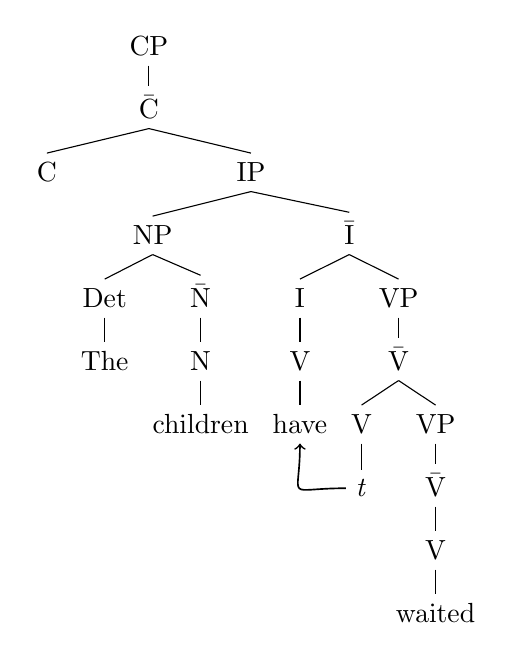
\begin{tikzpicture}
      \tikzset{level distance=8mm}
      \Tree [.CP [.\={C} C [.IP [.NP [.Det The ] [.\={N} [.N children ] ] ]
            [.\={I} [.I [.V \node(i){have}; ] ] [.VP [.\={V} [.V \node(t){\textit{t}}; ] [.VP [.\={V} [.V waited ] ] ] ] ] ] ] ] ]
      \draw[semithick,->] (t).. controls +(west:1) and +(south:1)..(i);
    \end{tikzpicture}
  \end{figure}
\end{frame}

\begin{frame}{Limits of Universal Grammar}
	\textbf{Criticism of this kind of analysis}
  \begin{itemize}
  \item Explicitely not empirical (at least by Chomsky)
    \begin{itemize}
    \item Against ``behaviourism'', focus on competence
    \item Tends to categorize everything in terms of recursive symbolic structures
    \item Good for English~-- what about Chinese? Pirah\~{a}? \textit{Conversational} English?
    \end{itemize}
  \item Computationally complex, cognitively\ldots{} difficult to explain
  \end{itemize}
\end{frame}

\begin{frame}{Pushing the Boundaries of Generative Grammar}
	\textbf{Language processing is basically an inverse problem:}
  \begin{itemize}
  \item \ex{Colorless green ideas sleep furiously}
  \item \ex{The Sally hugged him the Thomas}
  \item \ex{Time flies like an arrow}
  \item \ex{The apartment that the maid who the service had sent over was decorated}
  \item \ex{Keine Kopfverletzung ist zu harmlos um sie nicht zu ignorieren}
  \end{itemize}
\end{frame}

\begin{frame}{Representations of meaning}
	\textbf{Language is conveying mental state through symbols}
  \begin{itemize}
  \item Grammar is only an ``artifact'' to structure the transportation of mental state
    \begin{itemize}
    \item Or: only an instrument for performative utterance
    \end{itemize}
  \item Semantics from a cognitive perspective: meaning is\ldots
    \begin{itemize}
    \item perspectivic (relative to utterance context)
    \item dynamic (system changes with environment)
    \item encyclopedic (association with experiences \& culture)
    \item determined by usage (a system derived from concrete experience)
    \end{itemize}
  \end{itemize}
\end{frame}

\begin{frame}{Aspects of Cognitive Grammar}
	\textbf{Some cognitive approaches to semantics and grammar}
  \begin{itemize}
    \item How is meaning represented?
      \begin{itemize}
      \item \ex{Prototypes, radial networks, schemata, \ldots}
      \item \ex{Metaphor}
      \end{itemize}
    \item How is meaning expressed through form?
      \begin{itemize}
      \item \ex{Construction grammar, grammatical construal, usage-based grammar\ldots}
      \item \ex{Information structure}
      \end{itemize}
  \end{itemize}
\end{frame}

\begin{frame}{Information Structure (aka Information Packaging)}
	\textbf{Conveying more information beyond denotation}
  \begin{itemize}
  \item Intonation can focus different parts of an utterance
    \begin{itemize}
    \item \ex{John only introduced Bill to \emph{Sue}}
    \item \ex{John only introduced \emph{Bill} to Sue}
    \item \ex{John only introduced \emph{Bill} to \emph{Sue}}
    \item \ex{John only \emph{introduced} Bill to Sue}
    \end{itemize}
  \item Differences in meaning independent of linguistic form!
  \end{itemize}
\end{frame}

\begin{frame}{Information Structure (aka Information Packaging)}
	\textbf{Constructions that relate meaning in conversation\footnote{See Martin Hilpert's lectures:
    \protect\url{https://www.youtube.com/watch?v=PJecXZp_SYw}}}
\begin{itemize}
  \item Different pragmatic practices are associated with:
    \begin{itemize}
    \item \ex{As for John, he lost his wallet}
    \item \ex{What happened was that John lost his wallet}
    \item \ex{What John did was lose his wallet}
    \item \ex{It was John who lost his wallet}
    \item \ex{What John lost was his wallet}
    \end{itemize}
  \end{itemize}
\end{frame}

\begin{frame}{Construction Grammar}
	\textbf{Constructions everywhere}
  \begin{itemize}
  \item Constructions are patterns whose form or meaning is not strictly predictable from their
    components:
    \begin{itemize}
    \item \ex{He has whiffled my borogroves completely vorpal again}
    \item \ex{*The knife chopped the carrots into the salad}
    \end{itemize}
  \item Embedded items are \emph{coerced}:
    \begin{itemize}
    \item \ex{There was cat all over the road}
    \item \ex{She smiled herself an upgrade}
    \end{itemize}

  \end{itemize}
\end{frame}

\begin{frame}{Metaphors}
	\textbf{Not just arbitrary idioms and poetry!}
\begin{itemize}
  \item We understand things in terms of metaphor, and use it all the time\footnote{See
      \textit{Metaphors we live by} by John Lakoff}
  \item Abstract term = container
    \begin{itemize}
    \item \ex{An argument has a hole, has less substance, does not have content}
    \item \ex{To find something in an argument}
    \end{itemize}
  \item Argument = journey
    \begin{itemize}
    \item \ex{The content of the argument proceeds, path to the core of the argument, the direction
        has no substance}
    \end{itemize}

  \end{itemize}
\end{frame}


%//////////////////////////////////////////////////////////////////////
\sectionheader[What does theory have to do with NLP, at all?]{\textbf{Applications}}
\section{Practical Connections to NLP Applications}

% https://langsci-press.org/catalog/book/111
% https://scholar.google.com/scholar_url?url=http://www.academia.edu/download/31380659/vantrijp2013linguistic_assessment_criteria.pdf&hl=en&sa=T&oi=gsb-gga&ct=res&cd=0&d=8757869640222665985&ei=6_iWXpq6NMfAmAGj547QAg&scisig=AAGBfm2-ei3yMne0c9biGZ1SbQWI-mfaJA
% https://www.sci-hub.tw/10.1515/lingvan-2018-0070 (PDF)
% metaphor detection: a computation perspective (PDF)
% http://arxiv.org/pdf/1609.09019v1.pdf
% https://www.mitpressjournals.org/doi/pdfplus/10.1162/089120103322753356&hl=en&sa=T&oi=gsb-gga&ct=res&cd=0&d=15742121240912269262&ei=-wGXXuv1JJXGmAGqxoGwDA&scisig=AAGBfm1ovt2k8fe2r_pauAAxXlOs95xwrQ


%//////////////////////////////////////////////////////////////////////
\sectionheader[Next: ???]{\textbf{Thank You!}}

\end{document}
